% Chapter 2
\glsresetall % reset the glossary to expand acronyms again
\chapter{Background}\label{ch:Background}
Background

% Sections
\section{Examples}
text
\subsection{Sub Section}
text
\subsubsection{Sub Sub Section}
text

% Example Glossary
\noindent \gls{AI}

% Example Reference
\noindent thanks to OpenCV\cite{opencv}

% Example Figure
% reference this figure in the text using \ref{fig.testPlot}
\begin{figure}[!htbp]
	\centering
	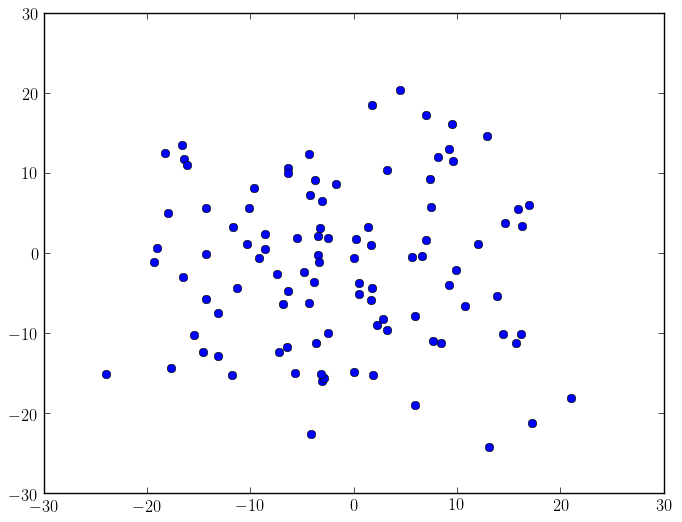
\includegraphics[width = 5in]{figs/testPlot.png}
	\caption{Test Plot}
	\label{fig.testPlot}
\end{figure}

% Example Equation
% I recommend using http://www.codecogs.com/latex/eqneditor.php to help make equations
% for tough equations or until you're familiar with LaTeX
% reference in the text using \ref{eqn.lowpassfilter}
\begin{equation}
	\mu_t = \alpha x + (1 - \alpha) \mu_{t-1}
	\label{eqn.lowpassfilter}
\end{equation}

% Example Nomenclature
\nomenclature{$\mu$}{Average}

% Example Code Listing
% reference in the text using \ref{ls.testPlot}
\lstset{language=python}
\lstset{tabsize=4}
\lstset{commentstyle=\color{blue}}
\lstset{frame=single}
\lstset{label = ls.testPlot}
\lstset{caption = Test Plot Code }
\lstinputlisting[float=!htbp]{figs/testPlot.py}

% Example Table
% I recommend using http://truben.no/latex/table/ to help with making tables
% reference in the text using \ref{tab.testTable}
\begin{table}[!htbp]
    \centering
    \begin{tabular}{|l|l|l|} % options are l,c,r (left, center, right)
    \hline
    ~ & ~ & ~ \\
    \hline
    ~ & ~ & ~ \\
    \hline
    ~ & ~ & ~ \\
    \hline
    ~ & ~ & ~ \\
    \hline
    \end{tabular}
    \caption{Test Table}
    \label{tab.testTable}
\end{table}
